\documentclass[]{article}
\usepackage[T1]{fontenc}
\usepackage[utf8]{inputenc}
\usepackage{color}
\usepackage{titlesec}
\usepackage{hyperref}
\usepackage{float}
\usepackage{datetime}
\usepackage{graphicx}
\usepackage{amsmath}
\usepackage{amsfonts}
\usepackage{attachfile}
\usepackage[margin=3cm]{geometry}
\graphicspath{{./resources}}
\hypersetup{
	colorlinks=true,
	linktoc=all,
	linkcolor=blue,
}

\title{Analysis of natural language complexity used by open-source developers\\ \large Introduction to Natural Language Processing}
\author{Komlichenko Ilya, Krzemiński Piotr, Monicz Kamil, \\Piotrowska Weronika, Wojnarowski Marcin}
\date{\monthname, \the\year}
	
\newcommand{\code}[1]{\texttt{#1}}
\newcommand{\figref}[1]{{(Fig. \hypersetup{linkcolor=blue}\ref{#1})}}

\begin{document}

\maketitle

{\hypersetup{linkcolor=black}\tableofcontents}
\newpage


\section{Motivation}

In order to improve our NLP skills, we are going to complete simple natural language analysis. The topic of choice should be close to our hearts so we stay engaged throughout the project. In addition, the source data should be freely accessible, so it is easy to work with. And so, our analysis will focus on the natural language complexity used by developers of various programming languages who contribute to open-source platforms (such as GitHub).

We hypothesize that language with a lower barrier of entry (such as Python) will exhibit a lower natural language complexity than languages that expect a higher level of expertise (such as C). Additionally, we are aware of different demographics of programming languages thus expect scientific/research focused languages (such as Julia) programmers will naturally use a more complex natural language to express ideas/problems.

In the end the following set of programming languages was chosen:

\begin{enumerate}
    \item Python
    \item C
    \item JavaScript
    \item Golang
\end{enumerate}

We believe this subset will represent a wide range of kinds of programmers: Python used by beginners/scientific community, C used by low level developers, JavaScript used by everyone, and Golang used by modern system's programmers. Thus they have a different target demographic so we believe it should show some noticeable differences. Another reason this subset was chosen is the availability of resources: these language are quite popular therefore much data is present for it in GitHub (discussed in greater detail in section \ref{scraping_procedure}).

\section{Data sourcing}

The linguistic data will be primarily scraped from the GitHub issues, where developers, using natural language, often describe bugs or feature requests related to some piece of software. And since the code there is publicly available, it is easy to assign a specific programming language to it.

\subsection{Text processing}

Every issue will be assigned a complexity/readability score based on industry-standard algorithms and bucketed into their respective programming language. For example, one could compute Flesch-Kincaid Grade Level or check the frequency of passive sentences.

\subsection{Scraping procedure} \label{scraping_procedure}

Using the official GitHub API we first fetch a list of users which we want to examine. To improve the quality of issues which we will be later studying, we made an assumption that GitHub users with more followers in general write issues of higher quality. We intuitively correlate higher followers count with a greater professionalism and higher activity on the platform. For each programming language a list of top 1000 (in terms of amount of followers) users with at least 170 followers\footnote{170 followers was chosen as the cutoff because it was the argmax such that all four programming languages have at least 1000 users each} was downloaded. An additional reason as to why the previously mentioned subset of languages was chosen is that these (unlike other languages which we had wished to investigate, such as purely scientific programming languages) do have a 1000 users with a reasonable amount of followers. Only personal accounts where taken into account, so organizations were filtered out since they represent more than a single person. A user was considered to be a $\mathbf P$ language programmer if majority of their repositories are written in $\mathbf P$\footnote{\href{https://docs.github.com/en/search-github/searching-on-github/searching-users\#search-by-repository-language}{Quoting the GitHub documentation}: "{\it \code{language:javascript} users [...] with a majority of their repositories written in JavaScript.}"}.

Afterwards, once we have a list of users (in total 4000 users) we proceed to fetching issues written by them. Top 100 issues created by a given user were downloaded. Only the body of the posted issue is saved, the thread that follows is ignored. Issues are ranked by the amount of interactions\footnote{An interaction consists of either a comment or a reaction} that they have received, thus top 100 issues refer to top 100 most active issues. Here, we make a similar assumption that more active issues correlate with a higher quality of natural language, for instance an RFC with naturally generates more traffic.

Finally, the gathered data is saved to a \code{csv} file containing the original author, their programming language, and the body of the issue. Since not every user had 100 issues, the final amount of scaped was 233,686 (where the upper bound is 400,000 if every user had 100 issues). We believe this is a very comfortable amount and even if after cleaning we will lose 50\%, this still will be enough.

\subsubsection{Technical details}

Scraper was written in the \href{https://www.rust-lang.org/}{Rust} programming language using the \href{https://github.com/XAMPPRocky/octocrab}{octocrab} library which wraps the official GitHub API. For all requests GitHub's search API was used, which has an unfortunate limit of 30 requests per minute. In each search call 100 items can be retrieved thus the whole scraping procedure spends $\frac{400000}{100 \cdot 30} = 133.(3)$ minutes on waiting for the limit rate alone. The scraper can be found in section \ref{attachments}.

\subsection{Cleaning up the data}

The previously scraped raw data contains a lot of noise, thus it has to be cleaned up. GitHub issues use markdown a text format which is a super-set of HTML, it allows for simple text formatting. Them being in a standardized format means we are able to parse them and work on their AST. For each body of an issue the following steps are taken:

\begin{enumerate}
    \item Parse into markdown AST
    \item Recursively walk the tree and skip tokens that are of non-interest (block code, inline code, links, images, etc.)
    \item Serialize the AST back to a visual rendered string form without the skipped tokens
\end{enumerate}

After these steps we are left with a much cleaner string representation of an GitHub issue. However, some additional steps have to be taken with the markdown cleaning due to limitation of the parsing markdown library and due to GitHub-specific features. Namely the following things were removed: hashtags (on GitHub they reference a different issue/pull request), unclosed code blocks, HTML comments (often appear in GitHub as issue templates), and inline URLs. Lastly we remove repetitive whitespace.

Now that we have clean utf-8 encoded text, we proceed to classify the content to its natural language. Since we are only interested in issues written in English we have to discard all issues written in a different natural language (for example chinese which was a common appearance). To do that a pre-trained model for Meta's \href{https://fasttext.cc/}{\code{fasttext}} NLP library. Given a string it classifies the natural language in which the text was written in. From there we filter in only those that were classified as english. Finally, if the cleanup content is not empty we save this entry into a new \code{csv} file.

Unfortunately, as we expected the final corpus is not perfect. Because of the human factor, we cannot guarantee that we removed all of the noise. For instance, someone could've written some code without wrapping it into code blocks or an inline code span. Thus we expect to still see some unwanted text in to final corpus. The dataset is unfortunately too large for us to manually clean it up. However we hope to be affected by these issues much less after choosing top users which should provide a higher quality of issues with regards to formatting. As seen on Fig. \ref{fig:cleaning-example} (in order of appearance) code blocks are removed, inline code is removed, non-english is discarded, and markdown formatting is removed to extract just the visual text.

\subsubsection{Technical details}

The data cleaner was written in Python using the previously mentioned library \code{fasttext}, standard dataframe tool \code{pandas}, and a markdown parser \code{mistletoe}. This process is much faster as it operates on local data. The data cleaner can be found in section \ref{attachments}.

\begin{figure}[H]
    \centering
    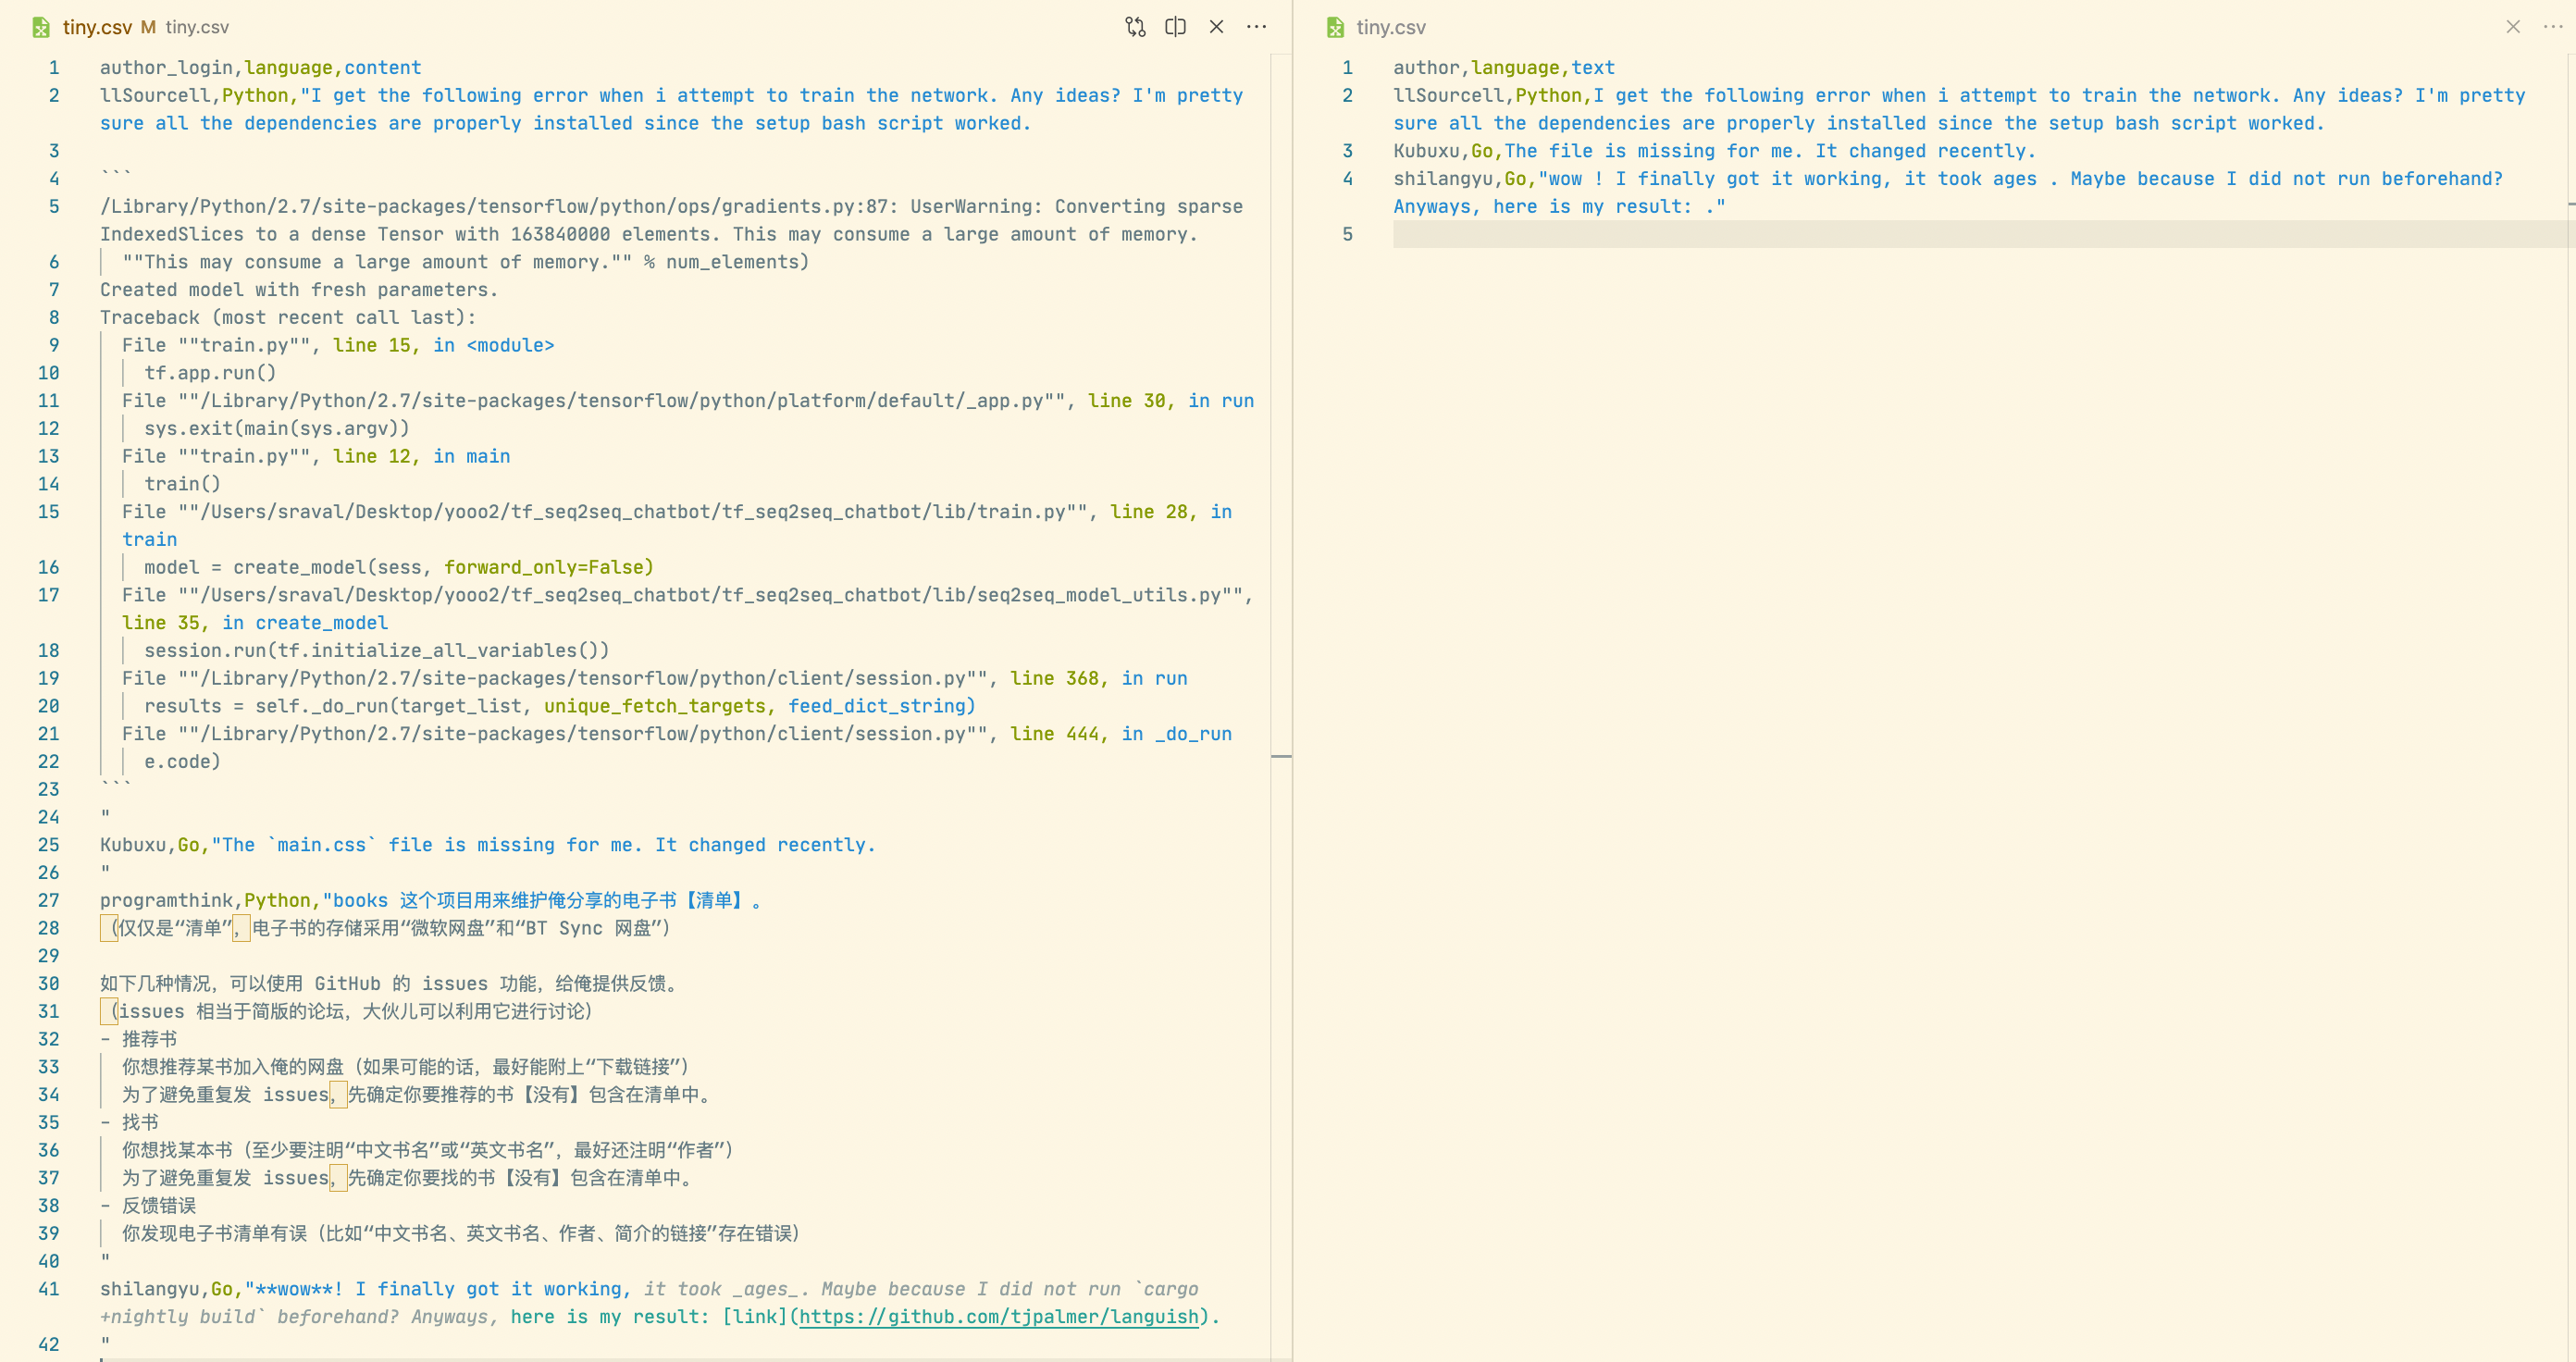
\includegraphics[width=1\textwidth]{cleaning-example.png}
    \caption{A sample example before (left) and after (right) cleaning of a csv file of the scraped issues.}
    \label{fig:cleaning-example}
\end{figure}

\subsection{Final corpus}

After cleaning we were left with 190643 instances, which means 18.4\% of instances were discarded. This is a very comfortable amount of data to make some analysis and draw some meaningful conclusions. On the other hand, the final corpus is as much as 67.2\% smaller (77MB vs. 235MB text csv) than the raw one, which shows that there was a lot of noise present and was successfully removed. But as mentioned before, there are still some false negatives left which we were able to identify when skimming the final corpus, thus it must be kept in mind during further analysis.

\section{Functionalities}

After scrapping the data, we are planning to perform following operations in order to give us a more complete insight

\begin{enumerate}
    \item Basic text analysis -- this includes average length of sentences, average length of words, most common word occurring etc. We are expecting developers of more complex programming languages to use more sophisticated language in the reported issues, this includes less grammar mistakes, longer sentences and words.

    \item Frequency of passive sentences -- in order to identify passive sentences we will use Part Of Speech tagging (POS). In English, a passive sentence can be defined by the place of the verb in the sentence and the form of this verb. We suspect the data to have high frequency of passive sentences, as it describes development issues.

    \item Flesh-Kincaid Grade Level -- by evaluating the Flesh-Kincaid grade level, we can determine whether the text is readable to an average, non-developer person. It measures the length of the sentences and syllables per words, which indicated the easy to read or not. We expect developers of more complex programming languages to write harder to read issue descriptions.

          \[0.39\left(\frac{\text{total words}}{\text{total sentences}}\right) + 11.8\left(\frac{\text{total syllables}}{\text{total words}}\right) - 15.59\]

    \item Flesh readability score -- similarly to Flesh-Kincaid Grade Level, this score is used to measure level of difficulty when reading a text. We compute the score as follows:

          \[206.835 - 1.015\left(\frac{\text{total words}}{\text{total sentences}}\right) - 84.6\left(\frac{\text{total syllables}}{\text{total words}}\right)\]
\end{enumerate}

We hope that after obtaining this data, there will be interesting conclusions that there exists dependency between a developer's primary programming language and the natural language he or she uses when describing issues on GitHub.

\section{Results}
\subsection{Basic text analysis}
\begin{enumerate}
    \item Average text length

          This graph presents average length of an issue description. We can observe that this value is similar for every analyzed language.


          \begin{figure}[H]
              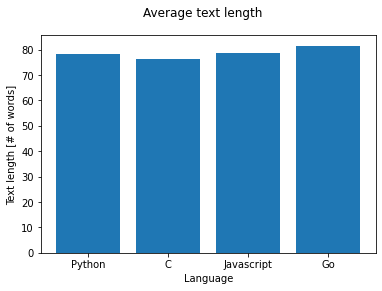
\includegraphics[width=8cm]{avg_len.png}
              \centering
          \end{figure}

    \item Average lexical diversity of a single issue

          This value is the average lexical diversity of a single issue. This value is obtained by dividing the set of tokens over the number of words in a single issue. The value is then averaged for each language. We can observe that this issue is similar among every language.

          \begin{figure}[H]
              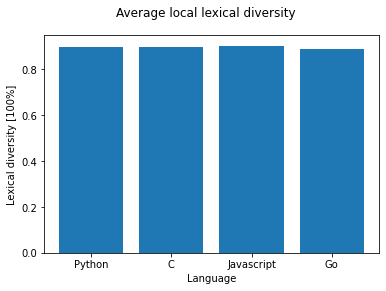
\includegraphics[width=8cm]{lex_div_single.png}
              \centering
          \end{figure}

    \item Total lexical diversity

          This value is the lexical diversity of all issues among the language. It is obtained by dividing set of tokens over number of all words in all issues. We can see that the lexical diversity is small for every language, which means all of the programmers write similar issue descriptions. However, C programmers tend to use the most diverse descriptions.

          \begin{figure}[H]
              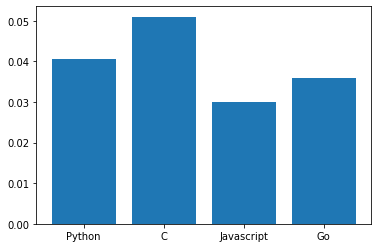
\includegraphics[width=8cm]{lex_div_total.png}
              \centering
          \end{figure}

    \item Average word length

          This is the average word length for every language. We can observe that this value is similar among all languages.

          \begin{figure}[H]
              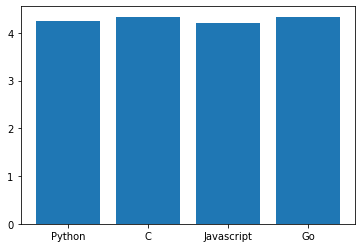
\includegraphics[width=8cm]{word_len.png}
              \centering
          \end{figure}

    \item Percentage of words over 10 characters

          Here is the percentage of words over 10 characters used in all issue descriptions among all languages. We can observe that all the programmers use long words with similar frequency.

          \begin{figure}[H]
              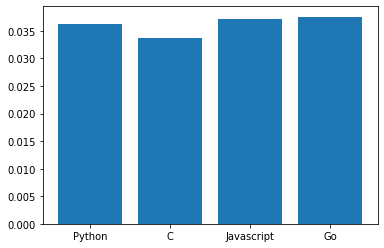
\includegraphics[width=8cm]{long_words.png}
              \centering
          \end{figure}

\end{enumerate}

\subsection{Frequency distributions}
In this section, we present the frequency distribution of tokens in the text. We can see the most common words used, as well as the cumulative value of this words.

\begin{enumerate}

    \item Python

          In Python, the most common words are would, like, code, use and using. Given over 2 900 000 tokens in the text, top 20 words make up to 37\% of the whole data.

          \begin{figure}[H]
              \includegraphics[width=8cm]{freq_Python.png}
              \centering
          \end{figure}

    \item C

          In C language, the most common words used are would, file, like, use and code. We can see that, given over 2 600 000 tokens in the text, top 20 words made up to 34\% of the total text.

          \begin{figure}[H]
              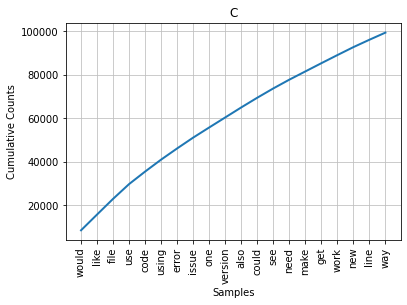
\includegraphics[width=8cm]{freq_C.png}
              \centering
          \end{figure}

    \item JavaScript

          In JavaScript, the most common words are would, like, use, using, could. Given 3 700 000 tokens in the whole text, top 20 words make up to over 40\% of the whole data.

          \begin{figure}[H]
              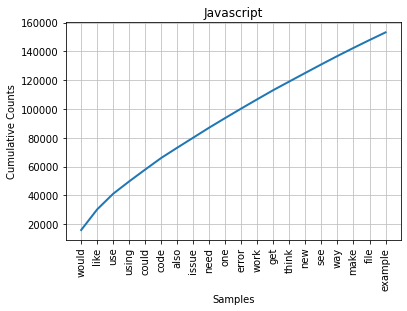
\includegraphics[width=8cm]{freq_java.png}
              \centering
          \end{figure}

    \item Golang

          In Go, most common words are would, like, go, use, using. Given over 4 500 000 tokens, the top 20 make up to 40\% of the whole text.

          \begin{figure}[H]
              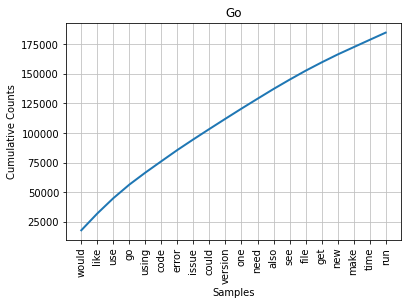
\includegraphics[width=8cm]{freq_Go.png}
              \centering
          \end{figure}


\end{enumerate}

We can observe that among all languages, issue comments contain variations of words would and use. The most informative feature is that C programmers use word "{\it file}" a lot, probably to low-level file access provided by C. Golang programmers use word "{\it go}" a lot, which may come from the language name.

\subsection{Frequency of passive sentences}

As expected, the frequency of passive sentences is high for all languages (in comparison to 10\% in most books), as it describes specific bugs in the code. One can see that C programmers use passive sentences the most, achieving almost 40\% of total passive sentences.

\begin{figure}[H]
    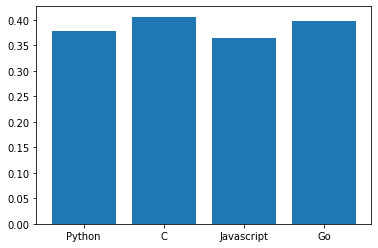
\includegraphics[width=8cm]{passives.png}
    \centering
\end{figure}

\subsection{Flesch readability score}

We can see that all of the languages fall into 60-70 interval, which leads them to be classified as easily understood by 13- to 15-year-old students. This score takes into account number of syllables per word and sentence length, which, as established earlier, was not high in most cases.

\begin{figure}[H]
    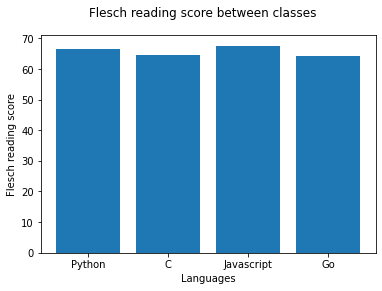
\includegraphics[width=8cm]{flesch.png}
    \centering
\end{figure}

\subsection{Flesch-Kincaid grade level}

In this case, all languages scored below 10, which makes them extremely difficult to read, understood only by university graduates. However this metric also takes into account number of words and syllables per sentence, it is much different than the previous Flesch metric. However, in most cases any text has higher Flesch reading score than Flesch-Kincaid grade level.

\begin{figure}[H]
    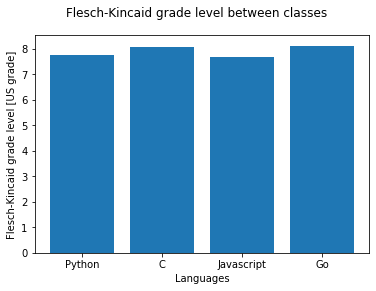
\includegraphics[width=8cm]{flesh_kincaid.png}
    \centering
\end{figure}

\section{Attachments} \label{attachments}

\begin{enumerate}
    \item %SCRAPER_ZIP%
    \item %DATA_CLEANER_ZIP%
\end{enumerate}


\end{document}
